\section{Интерференция волн от одного источника. Интерференционные опыты с делением волнового фронта (опыт Поля, бипризма Френеля, зеркала Френеля, билинза Бийе, зеркало Ллойда). Схема Юнга.}

\subsection{Интерференция волн от одного источника}


Для наблюдения интерференции света необходимо:
\begin{flushleft}
Постоянство во времени разности фаз складываемых колебаний


Равенство частот интерферирующих волн


Параллельность векторов \textbf{$E_1$} и \textbf{$E_2$}


Независимость от времени амплитуд световых волн.
\end{flushleft}

Если разность фаз двух колебаний с течением времени изменяется очень медленно, то говорят, что колебания остаются временно когерентными. \\ \\
Обозначим за $\tau$ время, за которое разность фаз двух колебаний успела измениться на величину, сравнимую $\pi$.\\ \\ За это время волна распространится на расстояние $c \tau$ , и колебания напряженности электрического поля волны в точках, удалённых друг от друга на это расстояние вдоль направления распространения волны оказываются некогерентными.\\ \\ Таким образом, расстояние вдоль направления распространения плоской волны, на котором случайные изменения разности фаз колебаний достигают величины, сравнимой с $\pi$, называют длиной когерентности (расстояние, при прохождении которого две или несколько волн утрачивают когерентность.)\\ \\

Наиболее распространённым способом получения двух когерентных волн является расщепление волны, излучаемой одним источником, на две волны, распространяющиеся по разным путям, но, в конце концов, встречающиеся в одной точке, где и происходит их сложение. Если запаздывание одной волны по отношению к другой, связанное с разностью пройденных ими путей, меньше длины когерентности, то колебания в точке сложения будут когерентными, и будет наблюдаться явление интерференции. Когда разность оптических путей двух волн приближается к длине когерентности, интерференционная картина исчезает, и интенсивность в каждой точке пространства становится равной сумме интенсивностей двух волн.

\subsection{Методы получения когерентных пучков}

Существующие экспериментальные методы получения когерентных пучков из одного светового пучка можно разделить на два класса.
\\ \\
В \textbf{методе деления волнового фронта} пучок пропускается, например, через два близко расположенных отверстия в непрозрачном экране.Такой метод пригоден лишь при достаточно малых размерах источника.
\\ \\
 В другом методе пучок делится на одной или нескольких частично отражающих, частично пропускающих поверхностях. Этот \textbf{метод деления амплитуды} может применяться и при протяженных источниках. Он обеспечивает большую интенсивность и лежит в основе действия разнообразных интерферометров. В зависимости от числа интерферирующих пучков различают двулучевые и многолучевые интерферометры. \\ \\ 
 
 \subsection{Схема Юнга}

\begin{center}
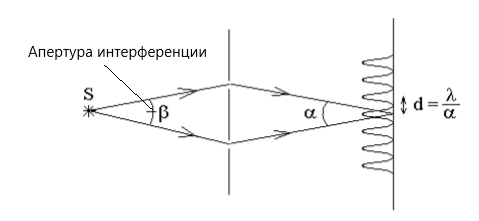
\includegraphics[scale = 0.7]{Yung}
\end{center}

Свет падает на экран с узкой щелью, дальше его можно рассматривать как точечный, монохроматический источника света $S$. После дифракции на щели световая волна распространялась до двух маленьких отверстий $S_1$ и $S_2$, сделанных в экране. После очередной дифракции два расходящихся пучка света перекрывают друг друга, и, являясь когерентными, при наложении дают интерференционную картину.

\subsection{Опыт Поля}

Опыт Поля - способ наблюдения интерференции света основанный на методу деления амплитуды.\\

В опыте Поля свет от источника S отражается двумя поверхностями тонкой прозрачной плоскопараллельной пластинки, в любую точку P, находящуюся с той же стороны от пластинки, что и источник, приходят два луча. Эти лучи образуют интерференционную картину. Для определения вида полос можно представить себе, что лучи выходят из мнимых изображений S1 и S2 источника S, создаваемых поверхностями пластинки. На удаленном экране, расположенном параллельно пластинке, интерференционные полосы имеют вид концентрических колец с центрами на перпендикуляре к пластинке, проходящем через источник S

\begin{center}
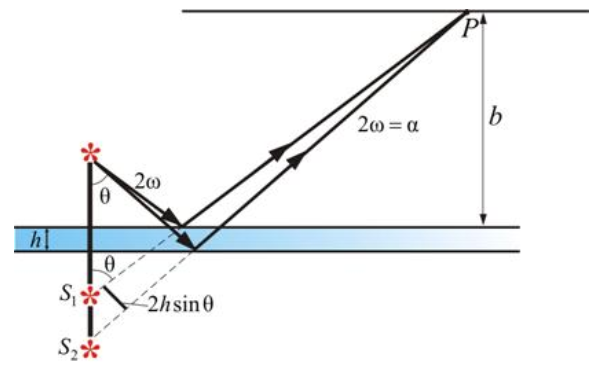
\includegraphics[scale = 0.5]{Pol}
\end{center}

\subsection{Бипризма Френеля}

Бипризма Френеля - призма, в основании которой находится тупоугольный равнобедренный треугольник.

\begin{center}
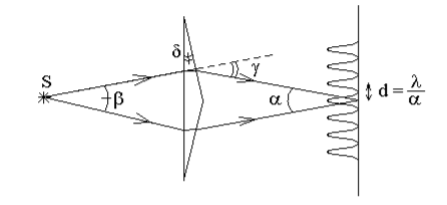
\includegraphics[scale = 0.5]{Biprizma}
\end{center}

Угол $\delta$ при основании треугольника и угол $\gamma$ , на который каждый из двух тонких оптических клиньев поворачивает луч, связаны соотношением:

$$\gamma = (n-1) \delta$$

\subsection{Зеркала Френеля}

Две когерентные световые волны получаются в результате отражения от двух зеркал $M$ и $N$, плоскости которых наклонены под небольшим углом $\phi$ друг к другу:
\begin{center}
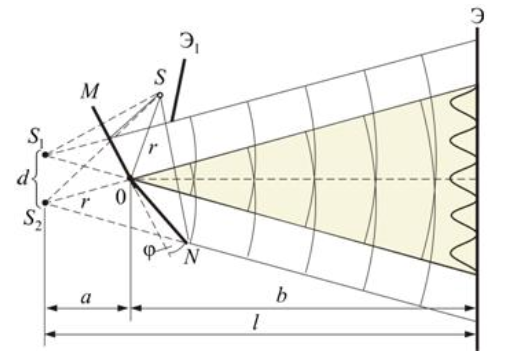
\includegraphics[scale = 0.5]{Zerkala}
\end{center}
Источником служит узкая ярко освещенная щель $S$, параллельная ребру между зеркалами. Отраженные от зеркал пучки падают на экран, и в той области, где они перекрываются (поле интерференции), возникает интерференционная картина. От прямого попадания лучей от источника $S$ экран защищен ширмой Э. Для расчета освещенности $J$ экрана можно считать, что интерферирующие волны испускаются вторичными источниками $S_1$   и  $S_2$, представляющими собой мнимые изображения щели $S$ в зеркалах. Поэтому $J$ будет определяться формулой двулучевой интерференции, в которой расстояние $l$ от источников до экрана следует заменить на  $a+b$ , где  $a \approx r$ - расстояние от S до ребра зеркал, $b$ - расстояние от ребра до экрана. Расстояние $d$ между вторичными источниками равно: $d \approx 2 a \phi$ . Поэтому ширина интерференционной полосы на экране равна:
$$ \Delta x \approx \frac{\lambda l}{d} = \frac{\lambda(a+b)}{2a \phi}$$

\subsection{Билинза Бийе}

Из обычной линзы вырезают полоску, получается билинза Бийе:

\begin{center}
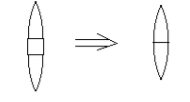
\includegraphics[scale = 0.5]{Bilinza1}
\end{center}

Точку пересечения фокальной плоскости и оси симметрии задачи можно назвать фокусом билинзы Бийе. Рассмотрим точечный источник света $S$, расположенный в фокусе билинзы Бийе и рассмотрим лучи света проходящие через верхнюю половину билинзы:

\begin{center}
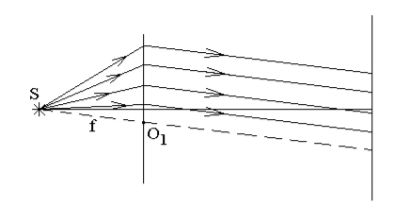
\includegraphics[scale = 0.5]{Bilinza2}
\end{center}

Если  верхнюю  половину  билинзы  достроить  вниз  до  полной  линзы,  то центр  полной  линзы  будет  находиться  в  некоторой  точке $O_1$,  расположенной ниже оси симметрии задачи.       Лучи,  прошедшие  через  верхнюю  половину  билинзы,  после  билинзы пойдут параллельно прямой $SO_1$, так как луч, проходящий через центр линзы $O_1$, должен пройти линзу без изменения направления. Остальные лучи обязаны быть параллельными лучу $SO_1$, так как источник света находится в фокальной плоскости. Как видно из рисунка этот пучок лучей наклонен вниз относительно оси симметрии задачи.       Аналогично, лучи, прошедшие нижнюю половину билинзы, пойдут после билинзы параллельным пучком лучей слегка наклоненным вверх.       На  экран  приходят  два  параллельных  пучка  лучей,  представляющих собой  две  плоских  волны.  Интерференционные  полосы  будут  иметь одинаковую ширину по всему экрану, так как угол между интерферирующими лучами в каждой точке экрана один и тот же.

\subsection{Зеркало Ллойда}

Интерферируют два луча, один идет прямо от источника света $S$ к экрану, второй отражается от зеркала, здесь $\beta$ - апертура интерференции. Ширина полос $ d = \frac{\lambda}{\alpha}$
\begin{center}
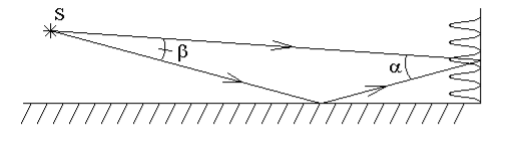
\includegraphics[scale = 0.5]{Loyd}
\end{center}
В нижней точке, где экран соприкасается с зеркалом, находится середина темной полосы. В эту точку волны приходят в противофазе, так как при отражении от зеркала одна из волн теряет половину волны.